\documentclass[12pt]{article}

\usepackage{fullpage}
\usepackage{multicol,multirow}
\usepackage{tabularx}
\usepackage{listings}
\usepackage{pgfplots}
\usepackage[utf8]{inputenc}
\usepackage[russian]{babel}
\usepackage{pgfplots}
\usepackage{tikz}

% Оригиналный шаблон: http://k806.ru/dalabs/da-report-template-2012.tex

\begin{document}

\section*{Лабораторная работа №8\, по курсу дискрeтного анализа: Динамическое программирование}

Выполнил студент группы М8О-312Б-22 МАИ \textit{Юрков Евгений}.

\subsection*{Условие}

\textbf{Вариант:} 1

Хитрый рюкзак

У вас есть рюкзак, вместимостью $m$, а так же $n$ предметов, у каждого из которых есть вес $w_i$ и стоимость $c_i$.
Необходимо выбрать такое подмножество $I$ из них, чтобы:
$$\sum_{i \in I} w_i \leq m$$
$$(\sum_{i \in I} c_i) * |I|$$
является максимальной из всех возможных.
$|I|$ – мощность множества $I$.


\textbf{Формат ввода:}
В первой строке заданы $1 \leq n \leq 100$ и $1 \leq m \leq 5000$.
В последующих n строках через пробел заданы параметры предеметов: $w_i$ и $c_i$.

\textbf{Формат вывода:}
В первой строке необходимо вывести одно число – максимальное значение $(\sum_{i \in I} c_i) * |I|$,
а на второй – индексы предметов, входящих в ответ.

\newpage
\subsection*{Метод решения}

Для решения задачи я воспользовался идеей, взятой из алгоритма классического рюкзака, дополнив её некоторыми условиями.
Я построил 3-хмерный массив $dp$, где $dp_{i j k}$ обозначало максимальную цену рюкзака весом $j$, в котором лежит ровно $k$ предметов,
которые были выбраны среди $i$ начальных предметов.

% \newpage
\subsection*{Описание программы}

Решение задачи находится полностью в функции \texttt{main}. Для удобства отладки была написана функция,
которая выводит в читаемом виде двумерную таблицу.

%\newpage
\subsection*{Дневник отладки}

Сначала я написал обычный рюкзак, но с другой формулой вычисления цены, однако этот алгоритм не учитывал все случаи.
Потом мне пришла идея сделать трёхмерный массив.

\newpage
\subsection*{Тест производительности}

Сложность алгоритма зависит от сложности заполнения массива $dp$, то есть его сложность $O(n^2 \cdot m)$
\begin{figure}
    \centering
    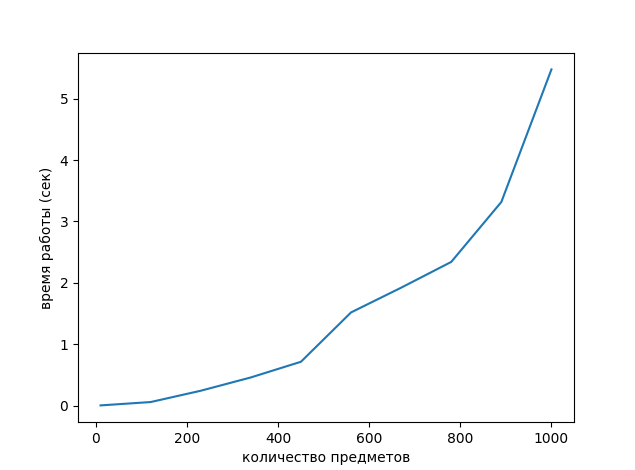
\includegraphics[width=\textwidth]{graph.png}
    \caption{График зависимости времени работы программы от количества предметов}
\end{figure}

% \newpage
\subsection*{Выводы}

В ходе данной лабораторной работы я изучил и применил методы динамического программирования на примере
задачи о рюкзаке с изменёнными условиями.

Эта работа научила меня эффективным методам решения оптимизационных задач, а также тому,
как динамическое программирование может быть адаптировано для решения задач с нестандартными условиями.
В процессе разработки сложность вызвало правильное построение трёхмерной таблицы и учёт всех зависимостей
между переменными, что потребовало аккуратного подхода к организации циклов и условий.

Полученные навыки могут пригодиться в различных областях, требующих оптимизации решений:
от анализа данных до разработки алгоритмов для сложных задач логистики или планирования ресурсов.
Понимание принципов динамического программирования и способность адаптировать их под различные условия
— важный инструмент для решения широкого спектра практических задач.
\end{document}